\documentclass{book}

% Packages to use
\usepackage{tabularx}
\usepackage{graphicx}
\usepackage{hyperref}
\usepackage{fontspec}
\usepackage{minted}

% Necessary Details 🤠
\title{Computer Scientist in A Nutshell}
\author{Miskatul Anwar}

% Font configuration
\setmainfont{IosevkaTermSlab Nerd Font}

% Starting the document

\begin{document}
\maketitle
%%%%%%%%%%%%%%%%%%%%%%%%%%%%%%%%%%% The book start from here
\newpage
\begin{flushright}
	Comming up \dots
\end{flushright}
\begin{itemize}
	\item  \textbf{Maths}
	      \begin{itemize}
		      \item Calculus
		      \item Differention \& Integration
		      \item Linear Algebra
		      \item Probability
	      \end{itemize}
	\item Java
	      \begin{itemize}
		      \item Setup
		      \item Setup
		      \item Compile \& Run
		      \item Basics
	      \end{itemize}
	\item \textbf{Python}
	      \begin{itemize}
		      \item Basics
		      \item Virtual Environment
		            \begin{itemize}
			            \item Python venv
			            \item Pyenv
			            \item Anaconda
		            \end{itemize}
	      \end{itemize}
	\item \textbf{R}
	      \begin{itemize}
		      \item Radiant
	      \end{itemize}
	\item  \textbf{Data Analysis}
	      \begin{itemize}
		      \item Numpy
		      \item Pandas
		      \item Matplotlib
	      \end{itemize}
	\item \textbf{Frameworks}
	      \begin{itemize}
		      \item Pytorch
	      \end{itemize}

	\item \textbf{Machine Learning}
	      \begin{itemize}
		      \item Supervised
		      \item Unsupervised
		      \item Reinforcement
	      \end{itemize}
	\item \textbf{Practice}
	      \begin{itemize}
		      \item Kaggle
		      \item CIFAR 10
		      \item EMNIST
	      \end{itemize}
	\item \textbf{Neural Network}
	      \begin{itemize}
		      \item Natural Language Processing(NLP)
		      \item Recurrent Neural Network(RNN)
	      \end{itemize}
	\item \textbf{Learn Generative AI}
	      \begin{itemize}
		      \item GPT Documentation
		      \item ChatGPT Short Courses
		      \item The GPT store
	      \end{itemize}
\end{itemize}


%%%%%%%%%%%%%%%%%%%%%%%%%%%%%%%%%%% Math
\chapter{Maths}

Maths will be the foundation what you'll need the most in this journey!
The most important topics are \dots

\section{Probability}

\begin{equation}
	P(H|E) = \frac{P(H) \cdot P(E|H)}{P(E)}
\end{equation}

P(H) = Probability  a  hypothesis  is  true\\
P(H)=Probability  of   seeing  the  evidence  if   the  hypothesis  is  true\\
P(E) = Probability   of   seeing   the   evidence\\
P(H|E) = Probability   a  hypothesis   is   true \\

The "|" stands for 'given'
P(H|E)  = P (Hypothesis \space given \space Evidence) \\
Also,
\begin{equation}
	P(H|E)=\frac{P(H \cap E)}{P(E)}\\
	\label{important}
\end{equation}
\begin{equation}
	P(E)P(H|E)=P(H \cap E)=P(H)P(E|H)\\
	\label{important2}
\end{equation}
\chapter{Java}
\section{Encapsulation}
Encapsulation is a fundamental concept in object-oriented programming (OOP) that binds together the data (variables) and the methods (functions)
that manipulate that data within a single unit, such as a class or module. This unit is designed to hide its internal details from the outside
world while exposing only necessary information through a controlled interface.\\
Why Encapsulation ?
\begin{enumerate}
	\item \textbf{Data Hiding}: Encapsulation helps to hide the implementation details of an object from the outside world, making it difficult for other parts of the program to access or modify the data directly.

	\item \textbf{Abstraction}: It provides abstraction by showing only the necessary information to the outside world while hiding the internal implementation details.

	\item \textbf{Code Organization}: Encapsulation promotes good code organization and structure by grouping related data and methods together.
\end{enumerate}
Ways to do that...
\begin{itemize}
	\item Java Packages
	\item Access Modifiers
	\item Java Encapsulation
	\item Data Hiding
	\item The `static` keyword
\end{itemize}
\subsection{Java Packages}
A package is simply a container that groups related types (Java classes, interfaces, enumerations, and annotations)
An example package:
\begin{figure}
	\centering
	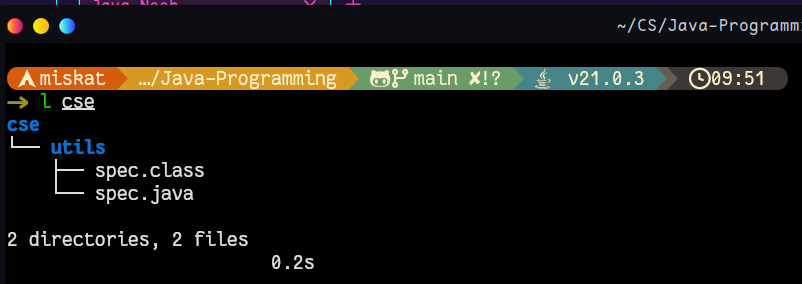
\includegraphics[width=0.45\textwidth]{../pngs/package.png}
	\caption{Linux Console}
\end{figure}

\subsection{Access Modifiers}
In Java, access modifiers are keywords that determine the visibility of a class, method, or variable to other parts of your program. They control
who can see or interact with these elements.
\begin{itemize}

	\item \textbf{public}: Accessible from anywhere in your program.
	\item \textbf{private}: Only accessible within the same class.
	\item \textbf{protected}: Accessible only within the same class and its subclasses.
	\item \textbf{default} (or no modifier): Accessible only within the same package.
\end{itemize}
Let's consider a simple example with a class `Car`:
\begin{minted}[frame=single]{java}
 public class Car {
    // public variable
    public String color = "red";

    // private method
    private void startEngine() {
        System.out.println("Vroom!");
    }

    // protected constructor
    protected Car(String make, String model) {
        this.make = make;
        this.model = model;
    }
}  
\end{minted}
\subsubsection{public}
\begin{itemize}
	\item Use public classes when you want to expose a class or interface to the outside world.
	\item Examples:
	      \begin{itemize}
		      \item  A web service API that needs to be accessed by clients.
		      \item  A utility class that provides common functionality.
	      \end{itemize}
\end{itemize}
\begin{minted}[frame=single]{java}
 public class MathUtils {
    public static int sum(int a, int b) {
        return a + b;
    }
}  
\end{minted}
\subsubsection{private}
\begin{itemize}
	\item Use private variables or methods when you want to hide internal implementation details from the outside world.
	\item Examples:
	      \begin{itemize}
		      \item A `Car` class might have a private `startEngine()` method that's not meant to be called directly by other classes.
		      \item An immutable class might have private setters and getters.
	      \end{itemize}
\end{itemize}

\begin{center}
	\begin{tabular}{|c|c|c|c|c|c|}
		\hline
		\textbf{Access Modifiers} & \textbf{Same Class} & \textbf{Same Package Subclass} & \textbf{Same Package Non-subclass} & \textbf{Different Package Subclass} & \textbf{Different Package Non-subclass} \\
		\hline
		\texttt{default}          & Y                   & Y                              & Y                                  & N                                   & N                                       \\
		\hline
		\texttt{private}          & Y                   & Y                              & N                                  & N                                   & N                                       \\
		\hline
		\texttt{protected}        & Y                   & Y                              & Y                                  & Y                                   & N                                       \\
		\hline
		\texttt{public}           & Y                   & Y                              & Y                                  & Y                                   & Y                                       \\
		\hline
	\end{tabular}
\end{center}

\subsection{Ways to Encapsulation}
\subsubsection{Simple Class}
A basic Java class that encapsulates a private integer variable \texttt{x} and provides a public method \texttt{getValue()} to retrieve its value:

\begin{minted}[frame=single]{java}
public class SimpleClass {
    private int x;

    public SimpleClass(int x) {
        this.x = x;
    }

    public int getValue() {
        return x;
    }
}
\end{minted}

\subsubsection{Bank Account}
A Java class that encapsulates a bank account, with private fields for balance and account number, and public methods to deposit, withdraw, and get the balance:

\begin{minted}[frame=single]{java}
public class BankAccount {
    private double balance;
    private int accountNumber;

    public BankAccount(int accountNumber) {
        this.accountNumber = accountNumber;
        this.balance = 0.0;
    }

    public void deposit(double amount) {
        balance += amount;
    }

    public void withdraw(double amount) {
        if (balance >= amount) {
            balance -= amount;
        } else {
            System.out.println("Insufficient funds!");
        }
    }

    public double getBalance() {
        return balance;
    }
}
\end{minted}

\subsubsection{Student Record}
A Java class that encapsulates a student's record, with private fields for name, age, and grades, and public methods to set and retrieve the information:

\begin{minted}[frame=single]{java}
public class StudentRecord {
    private String name;
    private int age;
    private double[] grades;

    public StudentRecord(String name, int age) {
        this.name = name;
        this.age = age;
        this.grades = new double[5];
    }

    public void setGrade(int index, double grade) {
        grades[index] = grade;
    }

    public double getAverageGrade() {
        double sum = 0.0;
        for (double grade : grades) {
            sum += grade;
        }
        return sum / grades.length;
    }
}
\end{minted}

\subsubsection{Use Cases}

\begin{enumerate}
	\item \textbf{Security}: Encapsulation ensures that sensitive data is protected from unauthorized access.
	\item \textbf{Code Reusability}: By encapsulating related data and methods, you can reuse the code in different parts of your program.
	\item \textbf{Improved Code Organization}: Encapsulation helps to organize your code in a logical and structured way.
\end{enumerate}

\subsubsection{Applications}

\begin{enumerate}
	\item \textbf{Database Management Systems}: Database management systems like MySQL or Oracle use encapsulation to hide their internal implementation details while providing a controlled interface for data manipulation.
	\item \textbf{Financial Applications}: Banking and financial applications, such as accounting software, use encapsulation to protect sensitive customer data and ensure secure transactions.
	\item \textbf{Gaming}: Games often use encapsulation to hide the internal workings of game mechanics, levels, or characters, making it easier to modify or extend the game without affecting other parts.
\end{enumerate}

In summary, encapsulation is a fundamental concept in object-oriented programming that helps to organize code, protect sensitive data, and improve code reusability.
\subsection{Data Hiding}
Data hiding is a principle of encapsulation that conceals the internal representation of an object's state (data) from external objects, making it difficult for other parts of the program to access or modify the data directly. This helps to:

\begin{enumerate}
	\item \textbf{Prevent Accidental Changes}: By hiding the internal state, you prevent accidental changes to the data from outside the class.
	\item \textbf{Control Access}: You can control access to the data by providing methods (getters and setters) that allow only authorized objects to modify the data.
	\item \textbf{Improve Code Quality}: Data hiding encourages good coding practices, such as using meaningful variable names and encapsulating related data.
\end{enumerate}

\subsubsection{How to Apply Data Hiding}

\begin{enumerate}
	\item \textbf{Make Data Private}: Declare the data variables as private within the class:
	      \begin{minted}[frame=single]{java}
    public class Example {
        private int x;
        // ...
    }
    \end{minted}

	\item \textbf{Use Getters and Setters}: Provide public methods (getters and setters) that allow controlled access to the data:
	      \begin{minted}[frame=single]{java}
    public class Example {
        private int x;

        public int getX() {
            return x;
        }

        public void setX(int value) {
            x = value; // validate or transform the value if needed
        }
    }
    \end{minted}

	\item \textbf{Avoid Direct Access}: Refrain from accessing the data directly from outside the class:
	      \begin{minted}[frame=single]{java}
    public class Example {
        private int x;

        public void someMethod() {
            System.out.println(x); // bad practice, avoid direct access
        }
    }
    \end{minted}
\end{enumerate}

\subsubsection{Best Practices}

\begin{enumerate}
	\item \textbf{Use Meaningful Variable Names}: Use descriptive names for your variables to make the code more readable.
	\item \textbf{Limit Access Modifiers}: Limit access modifiers (public, private, protected) to only what's necessary.
	\item \textbf{Validate Input}: Validate input data before modifying it to ensure integrity and prevent errors.
	\item \textbf{Use Immutable Objects}: Consider using immutable objects when possible, especially for sensitive or critical data.
\end{enumerate}

\subsubsection{Real-World Examples}

\begin{enumerate}
	\item \textbf{Bank Account}: A bank account class should hide its internal balance and only provide methods for depositing, withdrawing, and getting the balance.
	\item \textbf{Person Information}: A person information class might hide their personal details (name, age, address) and provide getter methods to access this information.
\end{enumerate}

By applying data hiding principles, you can create more robust, maintainable, and secure code that is easier to understand and modify over time.
\subsection{The `static` keyword}

The `static` keyword in Java is used to declare static variables or methods that belong to a class rather than an instance of the class. Here are
some key uses of the `static` keyword:
\begin{enumerate}
	\item  \textbf{Static Variables:} You can use `static` variables to store values that don't change throughout the program's execution.
	      \begin{minted}[frame=single]{java}

       public class MyMath {
    public static int MAX_VALUE = 100;

    public static void main(String[] args) {
        System.out.println(MyMath.MAX_VALUE); // prints 100
    }
  }
    \end{minted}
	\item  \textbf{Static Methods:} You can use `static` methods to perform operations that don't depend on instance-specific data.
	      \begin{minted}[frame=single]{java}
       
public class MathUtil {
    public static double sqrt(double num) {
        return Math.sqrt(num);
    }

    public static void main(String[] args) {
        System.out.println(MathUtil.sqrt(4)); // prints 2.0
    }
}
    \end{minted}
	\item\textbf{Singleton Pattern: }You can use `static` variables to implement the Singleton pattern, where only one instance of a class exists throughout
	      the program's execution.
	      \begin{minted}[frame=single]{java}
           public class Logger {
    private static Logger instance = null;

    public static Logger getInstance() {
        if (instance == null) {
            instance = new Logger();
        }
        return instance;
    }

    // ...
}
        \end{minted}
	      In this example, the `Logger` class uses a `static` variable to keep track of the single instance.
	\item \textbf{Utility Methods: } You can use `static` methods as utility methods that can be called from anywhere in your code without creating an instance
	      of the class.

	      Example:
	      \begin{minted}[frame=single]{java}
 public class StringHelper {
    public static boolean isEmpty(String str) {
        return str == null || str.trim().length() == 0;
    }

    public static void main(String[] args) {
        System.out.println(StringHelper.isEmpty("")); // prints true
        System.out.println(StringHelper.isEmpty("hello")); // prints false
    }
}          
        \end{minted}
	      In this example, the `isEmpty` method is a `static` utility method that can be called from anywhere in your code.

	      These are just a few examples of how you can use the `static` keyword in Java. Remember to use it wisely and only when necessary!
\end{enumerate}
\subsection{File Handling}

\textbf{Copying Contents from \texttt{INPUT.DAT} to \texttt{OUTPUT.DAT}}

\begin{minted}[frame=single]{java}
public class copyPaste {
    public static void main(String[] args) throws IOException {
        BufferedReader br = new BufferedReader(new FileReader("input.dat"));
        String str;
        if ((str = br.readLine()) != null) {
            System.out.println(str);
        }
        br.close();
        BufferedWriter bw = new BufferedWriter(new FileWriter("output.dat"));
        bw.append(str);
        bw.close();
        return;
    }
}
\end{minted}

\textbf{Using \texttt{DataOutputStream} and \texttt{DataInputStream}}

\begin{minted}[frame=single]{java}
import java.io.*;

public class file1 {
    public static void main(String[] args) throws IOException {
        FileOutputStream fout = new FileOutputStream("Test.txt");
        DataOutputStream out = new DataOutputStream(fout);
        out.writeDouble(98.6);
        out.writeInt(1000);
        out.writeBoolean(true);
        out.close();
        
        FileInputStream fin = new FileInputStream("Test.txt");
        DataInputStream in = new DataInputStream(fin);
        double d = in.readDouble();
        int i = in.readInt();
        boolean b = in.readBoolean();
        System.out.println("Here are the values: " + d + " " + i + " " + b);
        in.close();
    }
}
\end{minted}

\textbf{Reading from \texttt{output.txt}}

\begin{minted}[frame=single]{java}
import java.io.*;

public class file3 {
    public static void main(String[] args) throws IOException {
        BufferedReader br = new BufferedReader(new FileReader("output.txt"));
        String str;
        if ((str = br.readLine()) != null) {
            System.out.println(str);
        }
        br.close();
        return;
    }
}
\end{minted}


\subsection{\texttt{final} keyword in Java}

\begin{center}
	\begin{tabular}{|l|p{10cm}|}
		\hline
		\textbf{Type}  & \textbf{Description}                                                                                                                                                 \\
		\hline
		Final Variable & Variable with `final` keyword cannot be assigned again, similar to `const` in C. Once initialized, its value cannot be changed.                                      \\
		\hline
		Final Method   & Method with `final` keyword cannot be overridden by its subclasses. This ensures that the method's implementation in the superclass cannot be changed by subclasses. \\
		\hline
		Final Class    & Class with `final` keyword cannot be extended or inherited from. It serves as a final implementation that cannot be subclassed.                                      \\
		\hline
	\end{tabular}
\end{center}

\subsection{Java Inheritance}

\textbf{01 (Method Overriding)}

\begin{minted}[frame=single]{java}
// Parent class (Shape)
class Shape {
    void draw() {
        System.out.println("Drawing a shape");
    }
}

// Child class (Circle) that extends the parent class (Shape)
class Circle extends Shape {
    @Override
    void draw() {
        System.out.println("Drawing a circle");
    }
}

// Child class (Rectangle) that extends the parent class (Shape)
class Rectangle extends Shape {
    @Override
    void draw() {
        System.out.println("Drawing a rectangle");
    }
}

public class InheritanceExample1 {
    public static void main(String[] args) {
        // Create objects of the child classes
        Circle circle = new Circle();
        Rectangle rectangle = new Rectangle();

        // Use polymorphism to call the draw method on these objects
        Shape shape1 = circle;
        Shape shape2 = rectangle;

        shape1.draw();  // Output: Drawing a circle
        shape2.draw();  // Output: Drawing a rectangle
    }
}
\end{minted}

\textbf{02}

\begin{minted}[frame=single]{java}
// Parent class (Vehicle)
class Vehicle {
    void start() {
        System.out.println("Starting a vehicle");
    }
}

// Child class (Car) that extends the parent class (Vehicle)
class Car extends Vehicle {
    void accelerate() {
        System.out.println("Accelerating a car");
    }
}

// Child class (Motorcycle) that extends the parent class (Vehicle)
class Motorcycle extends Vehicle {
    void revEngine() {
        System.out.println("Revving a motorcycle engine");
    }
}

public class InheritanceExample2 {
    public static void main(String[] args) {
        // Create objects of the child classes
        Car car = new Car();
        Motorcycle motorcycle = new Motorcycle();

        // Use polymorphism to call the start method on these objects
        Vehicle vehicle1 = car;
        Vehicle vehicle2 = motorcycle;

        vehicle1.start();  // Output: Starting a vehicle
        vehicle2.start();  // Output: Starting a vehicle
    }
}
\end{minted}


\subsubsection{Using \texttt{super} keyword in Inheritance}

\begin{minted}[frame=single]{java}
class Animal {
    void sound() {
        System.out.println("The animal makes a sound");
    }
}

class Dog extends Animal {
    @Override
    void sound() {
        super.sound();
        System.out.println("Woof!");
    }
}

public class SuperKeywordExample {
    public static void main(String[] args) {
        Dog dog = new Dog();
        dog.sound();  // Output: The animal makes a sound, Woof!
    }
}
\end{minted}


\subsubsection{Using \texttt{this} keyword in Class}

\begin{minted}[frame=single]{java}
class Complex {
    int a, b;

    public Complex(int a, int b) {
        this.a = a;
        this.b = b;
    }

    void print() {
        System.out.println(a + " + " + b + "i");
    }

    Complex add(Complex num2) {
        Complex newnum = new Complex(a + num2.a, b + num2.b);
        return newnum;
    }
}

public class ThisKeywordExample {
    public static void main(String[] args) {
        Complex num1 = new Complex(11, 15);
        Complex num2 = new Complex(11, 15);
        num1.print();
        Complex res = num1.add(num2);
        res.print();
    }
}
\end{minted}

\subsection{Comparison: \texttt{this} vs. \texttt{super}}

\begin{center}
	\begin{tabular}{|p{0.45\linewidth}|p{0.45\linewidth}|}
		\hline
		\textbf{\texttt{this}}                                                                                                                                                                                                                                                     & \textbf{\texttt{super}}                                                                                                                                                                                                     \\
		\hline
		\texttt{this} is an implicit reference variable used to represent the current class. It can invoke methods of the current class and refer to its instance and static variables. It's also used to return and pass as an argument in the context of a current class object. & \texttt{super} is an implicit reference variable used to represent the immediate parent class. It can invoke methods of the immediate parent class, refer to its instance and static variables, and invoke its constructor. \\
		\hline
	\end{tabular}
\end{center}

\subsection{Constructors}

\textbf{01}
\begin{minted}[frame=single]{java}
class Innerconstructors {
    int a, b;

    public Innerconstructors() {
        a = 4;
        b = 7;
    }

    void print() {
        System.out.println(a + b);
    }
}

public class ConstructorsExample {
    public static void main(String[] args) {
        Innerconstructors num1 = new Innerconstructors();
        num1.print();
    }
}
\end{minted}

\textbf{02}
\begin{minted}[frame=single]{java}
class Innerconstructors {
    int a, b;

    public Innerconstructors() {
        a = 4;
        b = 7;
        System.out.println("New object created !");
    }

    void print() {
        System.out.println(a + b);
    }
}

public class ConstructorsExample {
    public static void main(String[] args) {
        Innerconstructors num1 = new Innerconstructors();
    }
}
\end{minted}

\textbf{03}
\begin{minted}[frame=single]{java}
class Innerconstructors {
    int a, b;

    public Innerconstructors(int real, int imaginary) {
        a = real;
        b = imaginary;
    }

    void print() {
        System.out.println(a + b);
    }
}

public class ConstructorsExample {
    public static void main(String[] args) {
        Innerconstructors num1 = new Innerconstructors(11, 15);
    }
}
\end{minted}

\textbf{04}
\begin{minted}[frame=single]{java}
class Innerconstructors {
    int a, b;

    public Innerconstructors(int real, int imaginary) {
        a = real;
        b = imaginary;
    }

    void print() {
        System.out.println(a + " + " + b + "i");
    }
}

public class ConstructorsExample {
    public static void main(String[] args) {
        Innerconstructors num1 = new Innerconstructors(11, 15);
        num1.print();
    }
}
\end{minted}

\subsubsection{Method Overloading}

\begin{minted}[frame=single]{java}
public class MethodOverloadingExample {
    void greetings() {
        System.out.println("Hello, Good Morning!");
    }

    void greetings(String name) {
        System.out.println("Hello " + name + ", Good Morning!");
    }
}
\end{minted}



\subsection{Possible ways to iterate \texttt{🏃}}

\textbf{\texttt{iterateInMap.java}}

\begin{minted}[frame=single]{java}
import java.util.ArrayList;
import java.util.HashMap;
import java.util.Map;

public class IterateInMap {
    public static void main(String[] args) {
        System.out.println("Ways to iterate in Map:");

        Map<String, Integer> tm = Map.of(
            "one", 1,
            "two", 2,
            "three", 3);

        // Method I
        for (Map.Entry<String, Integer> entry : tm.entrySet()) {
            System.out.println(entry.getKey() + " -> " + entry.getValue());
        }

        // Method II
        for (String key : tm.keySet()) {
            System.out.println(key + " -> " + tm.get(key));
        }

        // Method III
        for (Integer val : tm.values()) {
            System.out.println("Value: " + val);
        }

        // Method IV
        tm.forEach((key, value) -> System.out.println(key + " + " + value));
    }
}
\end{minted}

\subsection{\texttt{StringBuilders.java}}

\begin{minted}[frame=single]{java}
public class StringBuilders {
    public static void main(String[] args) {
        StringBuilder sb = new StringBuilder();
        sb.append("Hello");
        sb.append(", ");
        sb.append("World");

        System.out.println(sb.charAt(0));
        System.out.println(sb);

        for (int i = 0; i < sb.length(); i++) {
            sb.setCharAt(i, (char) (sb.charAt(i) + 1));
        }

        System.out.println(sb);
    }
}
\end{minted}

\subsection{The \texttt{Map} framework}

\subsubsection{\texttt{TreeMap} example}

\begin{minted}[frame=single]{java}
import java.util.TreeMap;

public class TreeMapExample {
    public static void main(String[] args) {
        TreeMap<String, Integer> hp = new TreeMap<>();
        hp.put("Bus", 2);
        hp.put("Car", 1);
        hp.put("Zeep", 1);
        hp.put("Plane", 1);

        System.out.println(hp);

        if (hp.containsKey("Bus")) {
            hp.putIfAbsent("Bus", 2);
        }

        if (hp.containsValue(2)) {
            System.out.println("Duo");
        }

        for (HashMap.Entry<String, Integer> e : hp.entrySet()) {
            System.out.println(e);
        }

        for (String key : hp.keySet()) {
            System.out.println(key);
        }
    }
}
\end{minted}

\subsubsection{\texttt{HashMap} example}

\begin{minted}[frame=single]{java}
import java.util.HashMap;

public class HashMapExample {
    public static void main(String[] args) {
        HashMap<String, Integer> hp = new HashMap<>();
        hp.put("Bus", 2);
        hp.put("Car", 1);
        hp.put("Zeep", 1);
        hp.put("Plane", 1);

        System.out.println(hp);

        if (hp.containsKey("Bus")) {
            hp.putIfAbsent("Bus", 2);
        }

        if (hp.containsValue(2)) {
            System.out.println("Duo");
        }

        for (HashMap.Entry<String, Integer> e : hp.entrySet()) {
            System.out.println(e);
        }

        for (String key : hp.keySet()) {
            System.out.println(key);
        }
    }
}
\end{minted}

\subsection{OMG \texttt{ArrayList}}

\textbf{\texttt{ArrayList} example}

\begin{minted}[frame=single]{java}
import java.util.ArrayList;

public class ArrayListExample {
    public static void main(String[] args) {
        ArrayList<Integer> list = new ArrayList<>();
        list.add(10);
        list.add(20);
        list.add(30);
        list.add(0, 30);

        for (Integer i : list) {
            System.out.println(i);
        }

        if (list.contains(10)) {
            System.out.println(list.toString());
        }
    }
}
\end{minted}

\subsection{Binary Search}

\textbf{\texttt{binarySearch1.java}}

\begin{minted}[frame=single]{java}
import java.util.ArrayList;
import java.util.Arrays;
import java.util.Collections;

public class BinarySearchExample {
    public static void main(String[] args) {
        ArrayList<Integer> num = new ArrayList<>(Arrays.asList(1, 2, 3, 4, 2, 1, 9, 8, 7, 2));
        Collections.sort(num);
        int target = 7;

        System.out.println("The target 7 found at index: " + Collections.binarySearch(num, target));
        System.out.println("Max : " + Collections.min(num));
        System.out.println("Min : " + Collections.max(num));

        Collections.sort(num, Collections.reverseOrder());
    }
}
\end{minted}

\subsection{Hot \texttt{Set}}

\textbf{\texttt{HashSet} example}

\begin{minted}[frame=single]{java}
import java.util.HashSet;

public class HashSetExample {
    public static void main(String[] args) {
        HashSet<Integer> s = new HashSet<>();
        s.add(4);
        s.add(1);
        s.add(1);
        s.add(2);
        s.add(3);

        System.out.println(s);
        System.out.println(s.contains(3));

        s.clear();
        System.out.println(s);
    }
}
\end{minted}

\textbf{\texttt{TreeSet} example}

\begin{minted}[frame=single]{java}
import java.util.TreeSet;

public class TreeSetExample {
    public static void main(String[] args) {
        TreeSet<Integer> set = new TreeSet<>();
        set.add(3);
        set.add(1);
        set.add(5);
        set.add(9);

        System.out.println(set);
    }
}
\end{minted}

\textbf{\texttt{LinkedHashSet} example}

\begin{minted}[frame=single]{java}
import java.util.LinkedHashSet;
import java.util.Iterator;

public class LinkedHashSetExample {
    public static void main(String[] args) {
        LinkedHashSet<Integer> s = new LinkedHashSet<>();
        s.add(4);
        s.add(2);
        s.add(1);

        System.out.println(s);

        Iterator<Integer> it = s.iterator();
    }
}
\end{minted}

\subsection{It's me bro :) \texttt{Stack}}

\textbf{\texttt{Stack} example}

\begin{minted}[frame=single]{java}
import java.util.Stack;

public class StackExample {
    public static void main(String[] args) {
        Stack<String> animals = new Stack<>();
        animals.push("Lion");
        animals.push("Dog");
        animals.push("Cat");
        animals.push("Rat");
        animals.push("Bat");

        System.out.println(animals);
        System.out.println(animals.peek()); // LIFO

        animals.pop();
        System.out.println(animals.toString());
    }
}
\end{minted}

\subsection{I'd like to be dynamic! \texttt{Heap}}

\textbf{\texttt{Queue} example}

\begin{minted}[frame=single]{java}
import java.util.LinkedList;

public class QueueExample {
    public static void main(String[] args) {
        LinkedList<Integer> queue = new LinkedList<>();
        queue.offer(12);
        queue.offer(24);
        queue.offer(36);

        System.out.println(queue);
        System.out.println(queue.peek());
        System.out.println(queue.element());

        queue.poll();
        System.out.println(queue);
    }
}
\end{minted}

\subsubsection{\texttt{Deque} example}

\begin{minted}[frame=single]{java}
import java.util.ArrayDeque;

public class DequeExample {
    public static void main(String[] args) {
        ArrayDeque<Integer> adq = new ArrayDeque<>();
        adq.offer(1);
        adq.offer(2);
        adq.offer(3);
        adq.offer(5);

        System.out.println(adq.peekFirst());
        System.out.println(adq.peekLast());
        System.out.println(adq);

        adq.poll();
        System.out.println(adq);

        adq.pollFirst();
        System.out.println(adq);

        adq.pollLast();
        System.out.println(adq);
    }
}
\end{minted}

\subsubsection{\texttt{PriorityQueue} example}

\begin{minted}[frame=single]{java}
import java.util.PriorityQueue;

public class PriorityQueueExample {
    public static void main(String[] args) {
        PriorityQueue<Integer> pq = new PriorityQueue<>();
        pq.offer(40);
        pq.offer(30);
        pq.offer(10);
        pq.offer(20);

        System.out.println(pq);
        System.out.println(pq.peek());
    }
}
\end{minted}

\chapter{Python}
Just try to learn the basics of python and that's it. Don't try to deep dive.
In 2024, learning something has become really easy. Understand the basics, keep your eye on the goal.
\begin{itemize}
	\item \href{https://youtu.be/rfscVS0vtbw?si=sfz5vdTybYIppFXz}{freecodecamp.org free course}
	\item \href{https://youtube.com/playlist?list=PLzMcBGfZo4-mFu00qxl0a67RhjjZj3jXm&si=2mE3gQfgFJAjnbJ3}{Tech With Tim Playlist}
\end{itemize}
\chapter{Data Analysis}
Some important \textit{Python} libraries for 'Data Analysis'...
\begin{itemize}
	\item Numpy
	\item Pandas
	\item Matplotlib
\end{itemize}
\section{Matplotlib}
\subsection{Basic Plotting}
\begin{minted}[frame=single]{python}
   
from numpy import *
from pylab import *

x = arange(-10, 10, 0.5)
y = x**2
plot(x, y, "r.")
show()
\end{minted}
\subsection{Scatter Plot}
\subsection{Histogram}
\subsection{Graphs}
\subsubsection{Mathematical Equations}
\begin{equation}
	f(x) = \sin(x)
\end{equation}
\begin{minted}[frame=single]{python}
   
import matplotlib.pyplot as plt
import numpy as np

ax = plt.axes()

# Plot for f(x) = sin(x)
# let's consider, y = f(x) = sin(x)

x_data = np.arange(0, 20, 0.1)
y_data = np.sin(x_data)

ax.set_title("f(x) = sin(x)", font="Maple Mono", color="red")
ax.set_xlabel("sin(x)")
ax.set_ylabel("sin(x)")
ax.plot(x_data, y_data)
plt.show()

\end{minted}

\subsection{3D Plotting}
\subsection{Surface Plot}
\textbf{Shpere}
\end{document}
